\documentclass[a4paper,11pt]{book}
\bibliographystyle{plain}
\usepackage[english]{babel}
\usepackage{textcomp}
\usepackage{fancyhdr}
\usepackage{makeidx}
\usepackage{tabularx}
\usepackage{graphicx}
\usepackage{parskip}
\usepackage{pdflscape}
\usepackage{floatflt}
\usepackage{ifthen}
\usepackage{background}
\makeindex
\pagestyle{fancy}
\fancyhf{}
\fancyhead[LE,RO]{\bfseries\thepage}
\fancyhead[LO]{\bfseries\rightmark}
\fancyhead[RE]{\bfseries\leftmark}
\renewcommand{\headrulewidth}{0.5pt}
\renewcommand{\footrulewidth}{0pt}
\addtolength{\headheight}{0.5pt}
\fancypagestyle{plain}{%
	\fancyhead{}
	\renewcommand{\headrulewidth}{0pt}
}
\usepackage[pdftex,pdfstartview=FitV]{hyperref}
\hypersetup{%
	pdftitle={Technical Report: LIMEFS Realtime File System},%
	pdfauthor={Rink Springer},
	pdfkeywords={LIMEFS Filesystem Realtime Linux}
}
\usepackage{draftcopy}
\usepackage[T1]{fontenc}
\usepackage[latin1]{inputenc}
\hyphenation{}
\setcounter{tocdepth}{3}
\setcounter{secnumdepth}{5}

% shortcut, used to define indexes words
\newcommand{\wi}[1]{\index{{#1}}{#1}}

% stand{on,off} is used to create a piece of text that 'stand out' of the
% current context
\newcommand{\standon}[2]{
	\vspace{5mm}
	\hrule
	\begin{sffamily}
	\textbf{\index{{#2}}{#1}}
}
\newcommand{\standoff}[0]{
	\end{sffamily}
	\vspace{5mm}
	\hrule
	\vspace{5mm}
}

% definities
\author{Rink Springer}
\title{Technical Report: LIMEFS Realtime File System}

\begin{document}

\frontmatter

% titel pagina
\begin{titlepage}
\hrule
\vspace*{\fill}
\begin{center}
{\Huge Technical Report} \\
\vspace{2cm}
\begin{figure}[htb]
\begin{center}
%\includegraphics[height=2cm]{delem_logo.jpg}
\end{center}
\end{figure}
LIMEFS Realtime File System\\
\vspace{2cm}
{\large Rink Springer}\\
\vspace{2cm}
Revision 1.1\\
\today\\
\vspace{2cm}
\end{center}
\vspace*{\fill}
\hrule
\end{titlepage}

% preface
\chapter{Preface}
\index{preface}

This report will describe my graduation internship at Philips Research in Eindhoven. It is written in an informative manner, with the exception of my personal evaluation which, of course, can't be objective or purely informative. The report is written using the guidelines as outlined in \cite{ROR}.

The goal of the internship was to design and implement a real time filesystem for Linux. This is illustrated further in the project description on page \pageref{project}.

The target audience is mostly people having an interest in the process or the execution of my internship. The technical documentation of the project is a separate document, which is included as appendix A. The project management plan, or \emph{plan van aanpak}, is included as appendix B.

Finally, I'd like to to thank the following people who helped me during my internship: Bas van Tiel, Michiel van Slobbe, Ron Eringa, Ad Denissen, Mischa Geldermans, Christ Vriens, Werner Almesberger and Wim Zijlmans.

Rink Springer \\
May 2005


\tableofcontents
\listoffigures

% summary
\chapter{Summary}
\index{summary}

This report provides an in-depth view of the technical aspects of the LIMEFS filesystem. It provides an extensive overview of the LIMEFS filesystem as well as a brief overview of the Linux Virtual File System design.

The following aspects are covered by this report:

\begin{itemize}
\item Linux I/O Layer \\
What is the basic design, what does a filesystem have to provide? Focuses mostly on the Linux Virtual File System layer.
\item LIMEFS \\
Overall design ideas of the LIMEFS filesystem, as well as all structures used within the LIMEFS filesystem.
\item Implementation \\
Linux Implementation-specific details of the filesystem.
\end{itemize}

The overall conclusion of the report is a stable filesystem which is very suitable for storing large files of a few gigabytes. There is room for improvement, especially within the administration part of the filesystem. As for most multimedia applications, the filesystem is ready to be used.


% definitions and abbreviations
\newcommand{\dodef}[2]{
	\index{{#1}}{#1}&{#2} \\
	\hline
}

\chapter{Definitions and abbreviations}
\label{defs}

\begin{tabularx}{\textwidth}{|l|X|}
\hline
\dodef{ABISS}{Active Block I/O Scheduling System, a scheduling system which can provide guaranteed read- and write I/O performance to applications \cite{ABISS}}
\dodef{dentry}{Directory entry, data structure (include/linux/dcache.h) in the directory cache which contains information about a specific inode within a directory}
\dodef{extent}{An (offset, length) pair}
\dodef{hard link}{A directory entry that directly references an inode. If there are multiple hard links to a single inode and if one of the links is deleted, the remaining links still reference the inode. \cite{TDaIotFOS}}
mmap(2), unlink(2)&These are references to C library functions. The number between parentheses defines the section number in the appropriate manual page \\
\hline
\dodef{inode}{A data structure used by the filesystem to describe a file. The contents of an inode include the file's type and size, the UID of the file's owner, the GID of the directory in which it was created, and a list of the disk blocks and and fragments that make up the file. \cite{TDaIotFOS}}
\dodef{LIMEFS}{Large-file metadata-In-Memory Extend-based File System, the filesystem created during the internship}
\dodef{soft link}{A file whose contents are interpreted as a path name when it is supplied as a component of a path name. Also called a soft link. \cite{TDaIotFOS}}
\dodef{symbolic link}{See soft link}
\end{tabularx}


\mainmatter

% 1. introduction
\chapter{Introduction}
\index{introduction}

This technical report describes the LIMEFS filesystem. This filesystem was written during my graduation project of my Computer Sciences study at Fontys Hogescholen in Eindhoven and carried out at Philips Research in Eindhoven. The goal was design and implement a framework for realtime file storage, which came down to implementing a realtime filesystem which can provide guaranteed I/O performance.

The report will provide a rough description of the Linux Virtual File System structure. The next part will focus completely on the design and implementation of the XXFS filesystem, followed by concluding statements on the project.


% 2. I/O layer overview
\newcommand{\prototype}[1]{
	\begin{tabularx}{\textwidth}{|l|X|}
	\hline
	Prototype&\texttt{#1} \\
	\hline
	\end{tabularx}
}

\chapter{Linux I/O Layer}

\section{Introduction}

This chapter will describe the Linux I/O layer. In order to develop a filesystem, you should understand how a Linux system interacts with files, devices and filesystems. This chapter will shed light on Linux I/O internals.

It is surprising to see how close Linux tries to follow the original UNIX architecture, as outlined in \cite{TDotUOS}. This book is a good reference to understand the algorithms and major design ideas (for example, of the cache code), but not the actual implementation.

Only the actual filesystem layer itself will be described in detail, because it is the most important for this project. For a complete overview of the I/O path, refer to Job Wildschut's technical graduation report: Linux IO Performance, which sheds light on the internals. \cite{LIOP}

\newpage

\section{Overview}

Linux I/O can be summarized in the following image:

\begin{figure}[h]
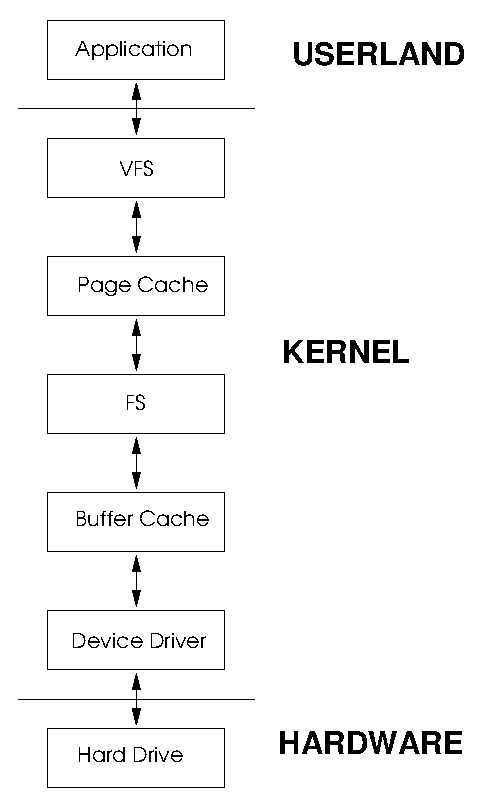
\includegraphics[height=10cm]{io-overview}
\caption{Summary of Linux I/O layers}
\end{figure}

Whenever a file is accessed, the request is passed down to the Virtual Filesystem. The VFS is actually a generic, filesystem independent interface which translates system calls, like open(2), read(2) etc to specific filesystem functions.

The page cache provides an uniform interface to file reading/writing, which handles functions like mmap(2). It provides all functionality in generic functions, relying only on the filesystem to provide buffers (using the buffer cache) for the actual data on disk. All other functionality is implemented by the filesystem code itself, described below.

The filesystem will receive VFS and page-cache requests and resolve them to I/O requests. These I/O requests are handled by the buffer cache, which will read blocks from a device and place them in a cache buffer. Modified buffers are written back to the disk as needed. The filesystem must conform to an interface as defined in the VFS layer. This layer is described in the VFS layer section later on.

The device driver is the device-dependent layer, which will handle the Linux I/O request and translate it into a device request.

\section{VFS layer}

This section will describe the VFS layer as well as the connection between the VFS and the page cache.

Before a filesystem is known by the kernel, it must be registered. This must be done using the \texttt{register\_filesystem()} call, which takes a \texttt{struct file\_system\_type} argument.

The most important member of this struct is \texttt{get\_sb} (get superblock), which points to a function which Linux will call whenever it tries to mount a filesystem of this type. This function must setup the \texttt{struct super\_block} which is passed along with it.

\subsection{Superblock operations}

\begin{verbatim}
static struct super_operations lime_sops = {
 .alloc_inode   = lime_alloc_inode,
 .destroy_inode = lime_destroy_inode,
 .read_inode    = lime_read_inode,
 .write_inode   = lime_write_inode,
 .put_super     = lime_put_super,
 .write_super   = lime_write_super,
 .statfs        = lime_statfs,
};
\end{verbatim}

The superblock operations structure contains the more low-level functions for a filesystem. These are basic operations such as inode management.

Dealing with files/directories will be done using the directory operations of the root inode (\texttt{sb-$>$s\_root} must always be set to the root inode), which will be covered in section \ref{dirops}.

\subsubsection{alloc\_inode}

\prototype{struct inode* alloc\_inode (struct super\_block* sb)}

Used to allocate an inode. The function should call the generic function \texttt{new\_inode} to allocate an inode and initialize it with filesystem-specific data.

\subsubsection{destroy\_inode}

\prototype{void destroy\_inode (struct inode* inode)}

The opposite of \texttt{alloc\_node}, this function must clean up the extra inode information. The inode itself must \emph{not} be destroyed, the VFS will take care of this.

\subsubsection{read\_inode}

\prototype{void read\_inode (struct inode* inode)}

Called whenever an inode structure must be filled, the inode to read is specified in \texttt{inode-$>$i\_ino}. Of all inode structure members, a few deserve special attention:

\texttt{inode-$>$i\_fop} is a pointer to an operations structure, which contains pointers to functions used for actual file/directory manipulation. These file operations are outlined in section \ref{fileops}, the directory operations can be found in \ref{dirops}.

\texttt{inode-$>$i\_op} is a pointer to an inode operations structure, which contains pointers to functions only needed for directory operations. These functions can be found in section \ref{inodeops}.

Should this operation fail, \texttt{make\_bad\_inode(inode)} must be used in order to invalidate the inode.

\subsubsection{write\_inode}

\prototype{void write\_inode (struct inode* inode, int synchronous)}

This will write inode data to the disk. The parameter indicates whether the data must be written synchronous, but is not implemented by most filesystems.

\subsubsection{put\_super}

\prototype{void put\_super (struct super\_block* sb)}

This will be called when the VFS unmounts the filesystem. Normally, a filesystem should update the on-disk superblock when the filesystem is dirty.

\subsubsection{write\_super}

\prototype{void write\_super (struct super\_block* sb)}

Called whenever the superblock needs to be written to the disk. This is for instance used while performing a sync(1) or fsync(2).

\subsubsection{statfs}

\prototype{int statfs (struct super\_block* sb, struct kstatfs* buf)}

Used to query used/free space/inode information. \texttt{struct kstatfs} can be found in \texttt{include/linux/statfs.h}, which must be filled by this function.

\subsection{Directory operations}
\label{dirops}

\begin{verbatim}
struct file_operations lime_dir_ops = {
 .read    = generic_read_dir,
 .readdir = lime_readdir,
 .fsync   = file_fsync,
};
\end{verbatim}

The functions outlined here are only used for directory inodes. Only \texttt{readdir} needs to be implemented (for it is very filesystem specific), the other functions call generic VFS functions which are suitable for most filesystems.

\subsubsection{readdir}

\prototype{int readdir (struct file* filp, void* dirent, filldir\_t filldir)}

Called to retrieve files in a directory (directory inode is \\
\texttt{filp-$>$f\_dentry-$>$d\_inode}), starting from offset \texttt{filp-$>$f\_pos}. This offset must be updated after new entries are passed, so the VFS knows which offset it must query to obtain the next directory entry.

\texttt{filldir} is the function to be called for each result, a prototype can be found in \texttt{include/linux/fs.h}.

\subsection{Inode operations}
\label{inodeops}

\begin{verbatim}
struct inode_operations lime_dir_inode_ops = {
 .create    = lime_create,
 .lookup    = lime_lookup,
 .link      = lime_link,
 .unlink    = lime_unlink,
 .symlink   = lime_symlink,
 .mkdir     = lime_mkdir,
 .rmdir     = lime_rmdir,
 .rename    = lime_rename,
};
\end{verbatim}
 
Misleading as the name may be, inode operations are mainly used in a directory context. They are mainly invoked for creating new inodes and looking up inode information. File inodes use so-called file operations which are outlined in section \ref{fileops}.

\subsubsection{create}

\prototype{int create (struct inode* dir, struct dentry* dentry, int mode, struct nameidata* nd)}

Creates a new file in \texttt{dir}, with name \texttt{dentry-$>$d\_name.name} and mode \texttt{mode}. On success, this function must call \texttt{d\_instantiate()} to add the created dentry to the cache.

\subsubsection{lookup}

\prototype{struct dentry* lookup (struct inode* dir, struct dentry* dentry, struct nameidata* nd)}

Called to retrieve the inode number from a filename (\texttt{dentry-$>$d\_name.name}) in a directory (directory inode is in \texttt{dir-$>$d\_ino}). On success, the inode found should be read (using \texttt{iget}) and added to the inode cache (using \texttt{d\_add}).

\subsubsection{link}

\prototype{int link (struct dentry* old\_dentry, struct inode* dir, struct dentry* dentry)}

Create a hard link from \texttt{old\_dentry} to \texttt{dentry} in directory \texttt{dir}. Inode information from \texttt{old\_dentry} can be copied over to the new inode as needed.

\subsubsection{unlink}

\prototype{int unlink (struct inode* dir, struct dentry* dentry)}

Removes an inode by name (\texttt{dentry-$>$d\_name.name}) in directory \texttt{dir}.

\subsubsection{symlink}

\prototype{int symlink (struct inode* dir, struct dentry* dentry, const char* symname)}

Create a soft link by name (\texttt{dentry-$>$d\_name.name}) in directory \texttt{dir}. The soft link should point to \texttt{symname}.

\subsubsection{mkdir}

\prototype{int mkdir (struct inode* dir, struct dentry* dentry, int mode)}

Create a new directory in parent directory \texttt{dir}. The directory name is passed in \texttt{dentry-$>$d\_name.name} and the mode in \texttt{mode}.

\subsubsection{rmdir}

\prototype{int rmdir (struct inode* dir, struct dentry* dentry)}

Removes directory named \texttt{dentry-$>$d\_name.name} from parent directory \texttt{dir}. This function must check whether the supplied directory is empty, and return \texttt{-ENOTEMPTY} if not.

\subsubsection{rename}

\prototype{int rename (struct inode* old\_dir, struct dentry* old\_dentry, struct inode* new\_dir, struct dentry* new\_dentry)}

This will rename entry \texttt{old\_dentry-$>$d\_name.name} in directory \texttt{old\_dir} to entry \texttt{new\_dentry-$>$d\_name.name} in directory \texttt{new\_dir}. This function must ensure \texttt{new\_dentry-$>$d\_name} doesn't already exist before continuing.

\subsection{File operations}
\label{fileops}

\begin{verbatim}
struct file_operations lime_file_ops = {
 .llseek     = generic_file_llseek,
 .read       = generic_file_read,
 .write      = generic_file_write,
 .mmap       = generic_file_mmap,
 .fsync      = file_fsync,
 .sendfile   = generic_file_sendfile
};
\end{verbatim}

These functions usually refer to generic VFS functions. All disk-based filesystems use the page cache for data reading/writing. The \texttt{generic\_file\_read} and \texttt{generic\_file\_write} functions use the inode's \texttt{i\_mapping-$>$a\_ops} to refer to the address space operations. These are documented below:

\begin{verbatim}
struct address_space_operations lime_aops = {
 .readpage      = lime_readpage,
 .writepage     = lime_writepage,
 .prepare_write = lime_prepare_write,
 .commit_write  = generic_commit_write
};
\end{verbatim}

The functions listed here use generic VFS calls, which ultimately only need a single function from the filesystem: the \texttt{get\_block} function, which is fully explained in \cite{TDotUOS}. A more Linux-specific explanation is given in the next paragraph.

\subsubsection{get\_block}

\label{getblk}
\prototype{int get\_block (struct inode* inode, sector\_t iblock, struct buffer\_head* bh\_result, int create)}

This function is passed to generic calls (these are \texttt{block\_read\_full\_page()} and \texttt{block\_write\_full\_page()}), which expects it to return a mapped buffer to a requested block within a file (the size of a block must be set on initialization time, using \texttt{sb\_set\_blocksize}).

The filesystem should allocate a new block if the the \texttt{create} flag is non-zero.

\section{ABISS}

\wi{ABISS}, or the Active Block I/O Scheduling System (as outlined in \cite{ABISS}) is a system designed to provide guaranteed read- and write performance to applications. The application issues a request to ABISS, in which a request is made for certain file bandwidth guarantees. ABISS will handle this by ordering writes and providing read-aheads as needed.

From a filesystem's point of view, some functions can be provided to ABISS, using the following structure:

\begin{verbatim}
struct abiss_fs_ops lime_fs_ops = {
 .get_block              = lime_do_get_block,
 .readpage               = lime_readpage,
 .alloc_unit             = lime_alloc_unit,
};
\end{verbatim}

The first function, \texttt{get\_block}, must be an entry point to the get block function as outlined in section \ref{getblk}. It is used to cache the logical block numbers, so no disk accesses are needed to look up blocks.

The second function, \texttt{readpage}, is the entry point to the file system's readpage function as outlined in section \ref{fileops}. This is used for the readahead functionality.

Finally, \texttt{alloc\_unit} must return the basic block allocation unit of the filesystem, in bytes.


% 3. limefs
\chapter{LIMEFS}
\index{LIMEFS}

\section{Introduction}

The LIMEFS filesystem contains a few distinctive characteristics:

\begin{itemize}
\item In-memory meta data \\
All \wi{meta data} used is in memory and stored consecutively on disk. This ensures fast updating, with few I/O operations. Most administration is built on-the-fly during mount time.
\item Few files/inodes \\
This filesystem is designed to store a few very large files. This makes a larger-than-normal data block size desirable.
\item Extent structure \\
Extents\footnote{An \wi{extent} is an ( offset, length ) tuple} are used to maintain data block administration.
\item Disk block size \\
The filesystem can use an user-defined block size, which is used for all I/O requests. This allows for good performance.
\item Inodes belong to directories \\
A directory is not a list of inodes residing in it. Each inode knows to which directory it belongs. Since all meta data is stored in-memory, this has barely any performance constraints.
\end{itemize}

The LIMEFS filesystem is designed to provide predictable performance.

Realtime I/O scheduling is not part of the filesystem. In order to have guaranteed disk I/O performance, the \wi{ABISS} framework is used. This framework can provide realtime I/O performance based on the application's wishes. ABISS itself is a separate project, more information can be found at \cite{ABISS}.

\section{Overview}

If we view a disk as an one-dimensional array of sectors, the next figure displays the on-disk structure:

\begin{figure}[h]
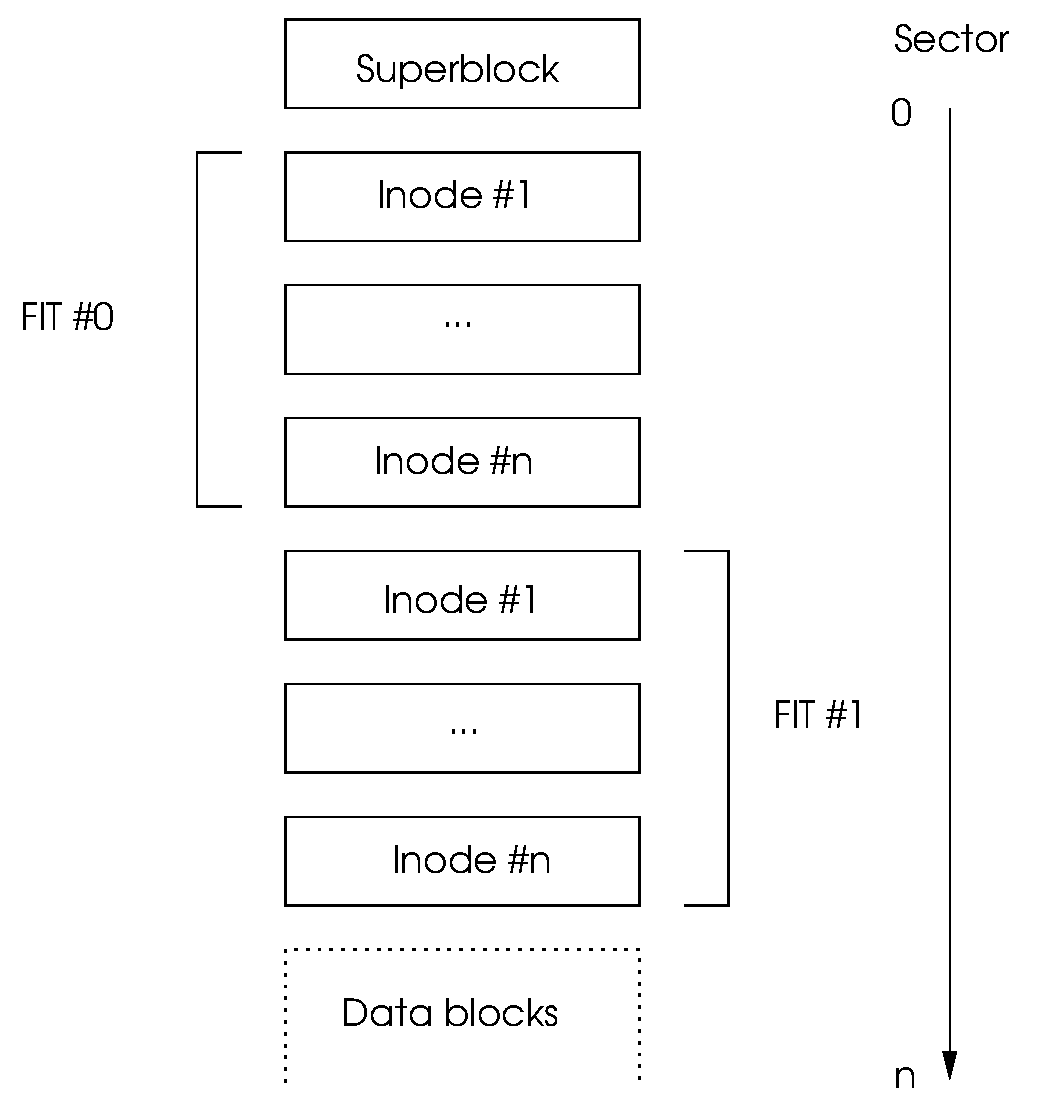
\includegraphics[height=8cm]{disk-layout}
\caption{On-disk structure of the filesystem}
\end{figure}

\begin{itemize}
\item Superblock \\
This is the very first filesystem structure. It contains read-only information needed to mount the filesystem.
\item File Information Table \\
The File Information Table, FIT, contains the inodes.
\item Data blocks \\
Space where the file data resides.
\end{itemize}

These structures will be explained in the next paragraphs.

\section{Superblock}
\label{superblock}

The \wi{superblock} contains a magic value used to identify the filesystem, as well as information used for mounting. The superblock is \emph{readonly}, and all values in it are copied to memory. This copy is used as long as the filesystem is mounted.

\index{struct!lime\_superblock}
\begin{verbatim}
struct lime_superblock {
 uint32_t sb_magic;
 uint32_t sb_version;
 uint32_t sb_diskBlockSize;
 uint32_t sb_dataBlockSize;
 uint64_t sb_numDiskBlocks;
 uint32_t sb_inodeSize;
 uint32_t sb_numInodes;
};
\end{verbatim}

\begin{tabularx}{\textwidth}{|l|X|}
\hline
sb\_magic&Magic value used for identification \texttt{LIME\_SB\_MAGIC (0xFC492B42)}\\
\hline
sb\_version&Current version number, \texttt{LIME\_SB\_VERSION (0x0001)}\\
\hline
sb\_diskBlockSize&Size of a disk block, in bytes. Due to Linux constrains, this may not exceed a page size (4KB on x86)\\
\hline
sb\_dataBlockSize&Size of a data block, in bytes. This must be a multiple of sb\_diskBlockSize.\\
\hline
sb\_numDiskBlocks&Total number of blocks on the disk (in sb\_diskBlockSize byte blocks)\\
\hline
sb\_inodeSize&Size of a single inode structure. Should be \texttt{1024} for version 1\\
\hline
sb\_numInodes&Total number of inodes on the filesystem, including reserved\footnote{reserved inodes are the root and checkpoint inodes} ones\\
\hline
\end{tabularx}

The next page will show an overview of the calculations with their corresponding place on the disk.

\newpage

Based on these values, calculations are made for often-used values:

\begin{displaymath}
fit\_in\_diskblocks = \frac{sbInodeSize * sbNumInodes + sbDiskBlockSize - 1}{sbDiskBlockSize}
\end{displaymath}
\begin{displaymath}
firstDataBlock = \frac{(1 + NUM\_FITS * fit\_in\_diskblocks) + \frac{sbDataBlockSize}{sbDiskBlockSize} - 1}{\frac{sbDataBlockSize}{sbDiskBlockSize}}
\end{displaymath}
\begin{displaymath}
numDataBlocks = \frac{sb\_numDiskBlocks}{\frac{sbDataBlockSize}{sbDiskBlockSize}} - firstDataBlock 
\end{displaymath}
\begin{displaymath}
fitOffset(n) = 1 + (n * fit\_in\_diskblocks)
\end{displaymath}

Graphically, this gives:

\begin{figure}[h]
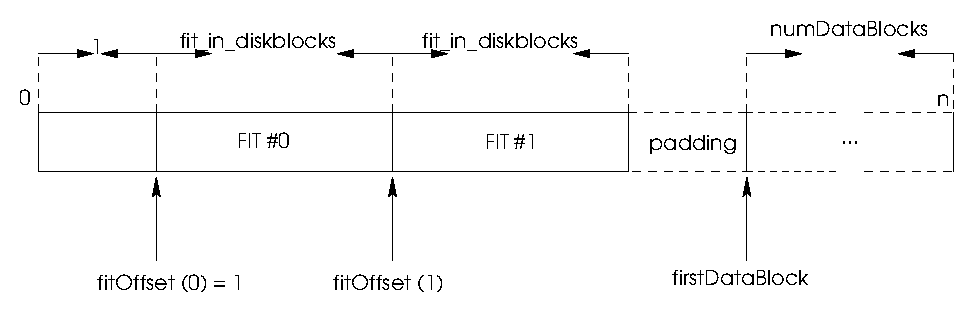
\includegraphics[width=12cm]{calc}
\caption{Internal offsets of on-disk structures}
\end{figure}

\section{File Information Table}
\label{fit}

A \wi{File Information Table} is an array of all inodes on the disk, and therefore spans numInodes entries (as defined in the superblock). The FIT is always stored two times; upon mount time, the filesystem reads the \wi{checkpoint inode} to find the most up-to-date copy.

\emph{Notice} Inode \#0 does \emph{not} exist within our filesystem. This is due to Linux having reserved this number (for example, it won't show up in directory lists). In order to work around this, we number our first inode \#1, which is always the \wi{root directory inode}.

\index{struct!lime\_inode}
\begin{verbatim}
#define LIME_MAX_NAME_LEN 256

struct lime_inode {
 uint32_t i_tag;                      /* type tag */
 uint32_t i_parentdir;                /* parent directory inode */
 char     i_name[LIME_MAX_NAME_LEN];  /* inode name */
 struct   lime_inode_data  i_idata;   /* posix data */
 union {
  struct  lime_file_inode  fi;
  struct  lime_dir_inode   di;
  struct  lime_hlink_inode hi;
  struct  lime_slink_inode si;
  struct  lime_checkpoint  ci;
  char    pad[739];
 } i_un;
};
\end{verbatim}

In order to store POSIX attributes, extra information must be stored on a per-inode basis. This information is represented by its own structure, and described below:

\index{struct!lime\_inode\_data}
\begin{verbatim}
struct lime_inode_data {
 uint16_t id_mode;     /* inode mode for protection */ 
 uint16_t id_uid;      /* user ID */
 uint16_t id_gid;      /* group ID */
 uint32_t id_atime;    /* last access time */
 uint32_t id_mtime;    /* last modification time */
 uint32_t id_ctime;    /* last status change time */
};
\end{verbatim}

\subsection{Directory Inode}

This inode describes a directory, which has no special characteristics. This is because the \texttt{i\_parentdir} field of each inode describes in which directory the inode resides.

\begin{figure}[h]
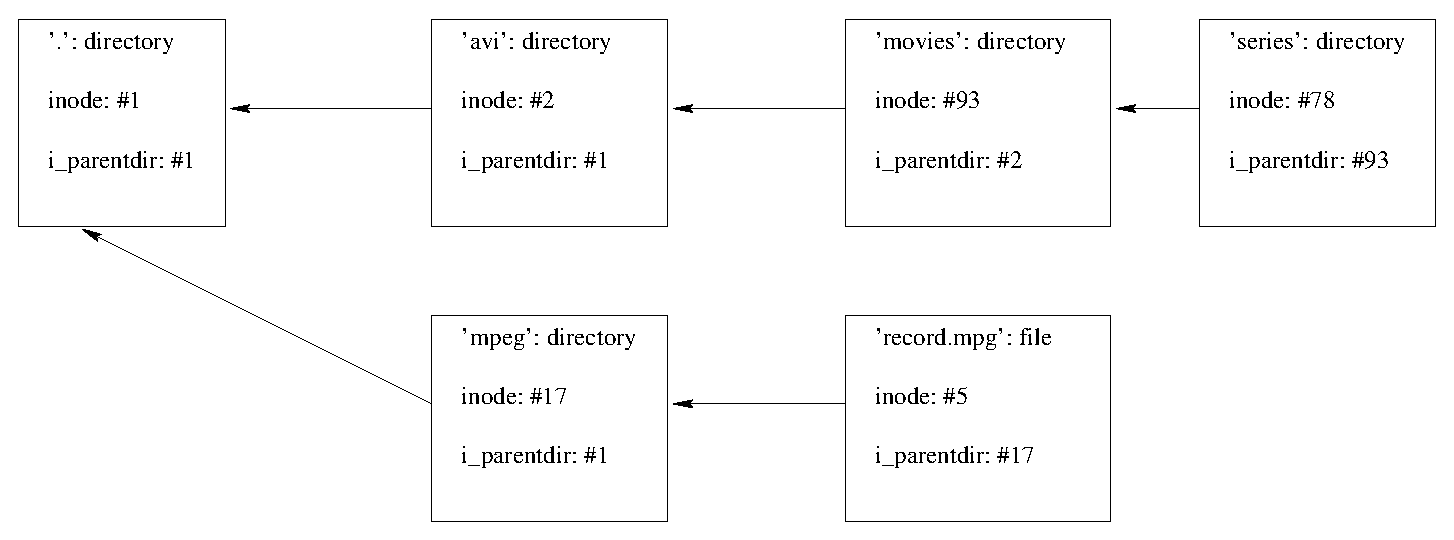
\includegraphics[height=5cm]{dir}
\caption{Nesting of directories}
\end{figure}

The tree for the figure is:

\begin{verbatim}
/
/avi
/avi/movies
/avi/movies/series
/mpeg
/mpeg/record.mpg
\end{verbatim}

\subsection{File Inode}
\label{fileinode}

An ordinary file, which contains data. The actual data blocks associated with the file are stored in \wi{extent} structures.

\index{struct!lime\_file\_inode}
\begin{verbatim}
#define LIME_EXTENTS_PER_INODE 80

struct lime_file_inode {
 uint32_t fi_boff;
 uint32_t fi_eoff;
 uint32_t fi_numextents;
 struct   lime_extent fi_extents[LIME_EXTENTS_PER_INODE];
};
\end{verbatim}

\begin{tabularx}{\textwidth}{|l|X|}
\hline
fi\_boff&Begin offset within the first extent \\
\hline
fi\_eoff&End offset within the last extent \\
\hline
fi\_numextents&Number of extents used \\
\hline
fi\_extents&Structure used to store the extents \\
\hline
\end{tabularx}

As stated in the definitions on page \pageref{defs}, an extent is simply a (offset, length) tuple. It contains the block offset, and the number of blocks used from this offset onwards.

\newpage

% let the text stand out a bit more
\standon{Fragmentation study}{fragmentation!study}

As can be seen, we allow a maximum of 80 extents per file. If more extents are needed than this maximum, the file cannot be expanded beyond the current size.

In order to determine how much of an issue this is, Ad Denissen and I created a small tool which simulates an extent-based 250GB filesystem with 4MB data blocks. It simulates writing 10.000 files sized between 500 and 5000MB. If a file does not fit, it will delete an existing one at random to take fragmentation into account. Finally, we refuse to allocate the last 5\% of the data blocks in order to decrease fragmentation\footnote{This value is based on some tests to determine an acceptable value}.

Plotting an overview of the number of fragments per file and the average fragmentation gives an interesting result:

\begin{center}
\begin{figure}[h]
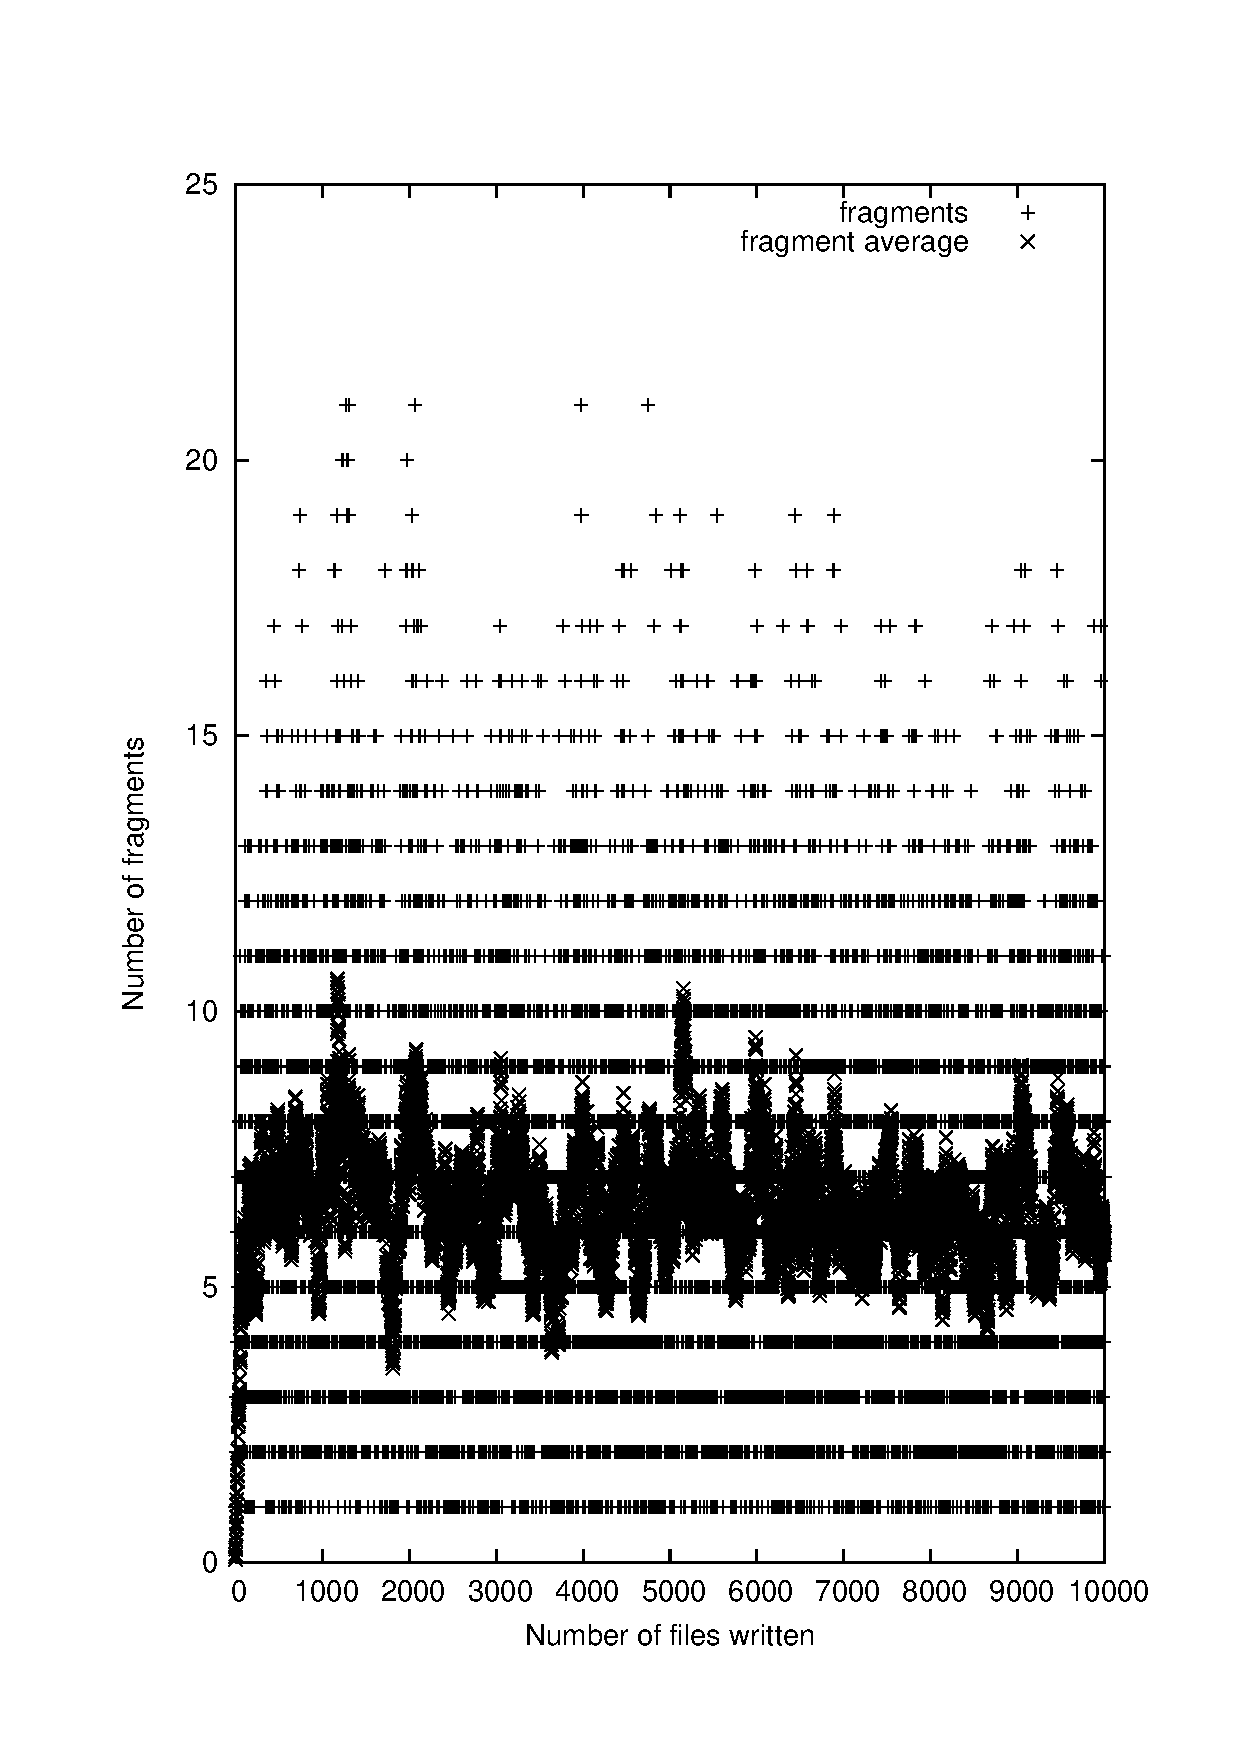
\includegraphics[width=7.5cm]{frag-log}
\caption{Fragments per file}
\end{figure}
\end{center}

As can be seen, the number of fragments never exceeds 21. This indicates the 80 extents we have is acceptable. However, it is also interesting to see the relationship between fragment sizes and the occurrence between them. 

In order to display this, we plot the fragment size as \emph{X} and the occurrence in \% as \emph{Y}. This gives the following result:

\begin{figure}[h]
\includegraphics[width=7.5cm]{frag-occurence}
\caption{Fragment occurrence}
\end{figure}

As can be seen in these images, huge fragments are quite rare, even in everyday usage.

\standoff

The extent structure is defined as:

\index{struct!lime\_extent}
\begin{verbatim}
struct lime_extent {
 uint32_t ex_offset;
 uint32_t ex_length;
};
\end{verbatim}

Extents always point to the data blocks and will be expanded if more space is needed (refer to section \ref{allocation} for more information). There is a hard limit on how many extents a file can have (\texttt{LIME\_EXTENTS\_PER\_INODE}), therefore a file can always consist of a minimum of \\
$LIME\_EXTENDS\_PER\_INODE * sbBlockSize$ bytes.

As can be expected, the filesystem will always attempt to expand the last extent. More information about the block allocation can be found in section \ref{allocation} on page \pageref{allocation}. The figure below shows an example of extent administration:

\begin{figure}[h]
\includegraphics[width=10cm]{file-extent}
\caption{File-extent administration}
\end{figure}

\label{offs}As stated above, \texttt{boff} and \texttt{eoff} are offsets within the first and last block. Refer to the image below:

\begin{figure}[h]
\includegraphics[width=10cm]{file-offs}
\caption{File begin- and end offsets}
\end{figure}

There are some implementation specific limitations on this approach, please refer to section \ref{impl_offs} for more information.

Based on these two offsets, the file size can be calculated in bytes as:

\begin{displaymath}
filesize = dataBlockSize \cdot \left( \sum_{i=0}^{n} ext(i)_{length} \right) - boff - \left( dataBlockSize - eoff \right)
\end{displaymath}

\subsection{Hardlink Inode}
\label{hardlink}

A \wi{hard link} is a reference to an inode, using a different name. Unlike traditional UNIX filesystems like FFS and ext, this filesystem allocates an extra inode with the hard link's name, but returns the destination inode. Therefore, we can implement this by simply storing the destination inode number.

\begin{figure}[h]
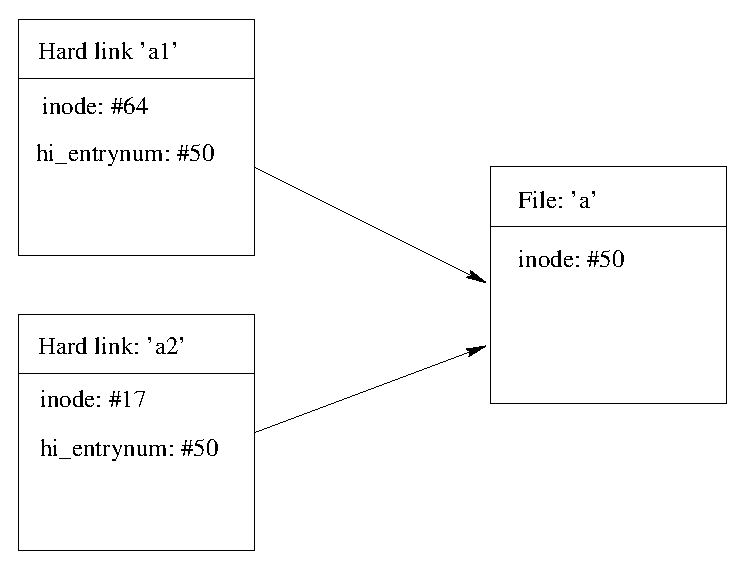
\includegraphics[height=5cm]{hard-link}
\caption{Hard link and file relationship}
\end{figure}
\index{struct!lime\_hlink\_inode}

\begin{verbatim}
struct lime_hlink_inode {
 uint32_t hi_entrynum;
};
\end{verbatim}

The implementation-specific notes can be found in section \ref{impl_hardlinks}.

\subsection{Softlink Inode}

A \wi{soft link}\footnote{also known as a symbolic link} is a reference to another location. It references by name, so therefore the destination doesn't have to be on this filesystem or even exist for that matter.

\index{struct!lime\_slink\_inode}
\begin{verbatim}
#define LIME_MAX_SYMLINK_LEN 256

struct lime_slink_inode {
 char si_path[LIME_MAX_SYMLINK_LEN];
};
\end{verbatim}

The soft link implementation is simple: all that needs to be done, is to pass the \texttt{si\_path} to the Linux VFS layer. This will resolve it to a new request to the accompanying filesystem.

\subsection{Checkpoint Inode}

The \wi{checkpoint inode} is used to determine the most recent copy of the FIT. It is always the final entry of the FIT; this increases the chance all entries are written before this final inode and thus are up-to-date.

\index{struct!lime\_checkpoint}
\begin{verbatim}
struct lime_checkpoint {
 uint32_t ci_followup;
};
\end{verbatim}

The followup count should only differ by 1, since they are used in a round-robin fashion. This means the FIT following the currently active FIT will be used. If the difference is not exactly one, the filesystem will not be mounted.

\section{Data blocks}

The data blocks start after the final File Allocation Table and are always aligned on a data block. They will continue until the end of the disk. The list of free blocks is constructed upon mount time, refer to section \ref{freespace} for more information.


% 4. implementation
\chapter{Implementation}
\index{implementation}

\section{Allocation}
\label{allocation}

As for any filesystem, \wi{fragmentation} hurts performance and therefore is preferably kept at a minimal level. This is especially true for our filesystem, since we have a maximum number of extents which can be stored within an inode, as outlined in section \ref{fileinode}.

In order to work around this, we use a different allocation strategy:

\begin{itemize}
\item Random first blocks \\
For every first file block, we take a random block somewhere within the free space list of our disk.
\item Extend previous blocks \\
If we have a previously allocated block, we try to take the next block. If this fails, we take a random block.
\end{itemize}

Support we have the layout as below, \emph{a} and \emph{b} are files. The text below the image is the extent map as stored within the FIT:

\begin{figure}[h]
\includegraphics[width=10cm]{alloc1}
\caption{Allocation strategy: initial status}
\end{figure}

Now, let's assume we allocate an extra block for file \emph{a}. Since there is a free block coming ahead, we can easily expand the extend. This gives the following:

\begin{figure}[h]
\includegraphics[width=10cm]{alloc2}
\caption{Allocation strategy: after extending file 'a'}
\end{figure}

However, suppose file \emph{a} wants another block. It may not overwrite the blocks already in use by file \emph{b}, so we allocate a random block:

\begin{figure}[h]
\includegraphics[width=10cm]{alloc3}
\caption{Allocation strategy: after extending file 'a' again}
\end{figure}

Finally, let's assume we create a new file, \emph{c}, with a single block. This block will be randomly put somewhere on the disk:

\begin{figure}[h]
\includegraphics[width=10cm]{alloc4}
\caption{Allocation strategy: new file 'c' with a data block}
\end{figure}

As can be seen, this hinders file \emph{a} since it cannot extend to the next block and thus must create a new extent.

\section{Free space}
\label{freespace}

\subsection{Introduction}

Unlike most traditional filesystems, LIMEFS does not store an overview of free blocks on the disk. Rather, this list is constructed upon mount time and consists of the following characteristics:

\begin{itemize}
\item Stored as an extent list \\
In order to allow quick access, the freelist is stored as an extent-based list.
\item Numerically sorted \\
The list is always numerically sorted. This simplifies merging adjacent blocks.
\item Limited number of entries \\
The maximum list size\footnote{This will happen if even numbered blocks are used whereas odd numbered blocks are free} is $\frac{numDataBlocks}{2}$. Tests have shown this never happens, so we use a tenth of the maximum, or $\frac{numDataBlocks}{10}$.
\end{itemize}

These characteristics will be illustrated in the next paragraph.

\subsection{Example}

Below is an example of a free list. Shaded blocks lines are allocated, blank blocks are available:

\begin{figure}[h]
\includegraphics[width=12cm]{freelist1}
\caption{Freelist: initial status}
\end{figure}

Now, we free block 3. This means we need to add an extra entry to our freelist (since it is in the middle of used blocks. This gives the following:

\begin{figure}[h]
\includegraphics[width=12cm]{freelist2}
\caption{Freelist: freed block 3, gives new extent}
\end{figure}

\newpage

Block ranges can also be extended. For example, if we free block 6, we get:

\begin{figure}[h]
\includegraphics[width=12cm]{freelist3}
\caption{Freelist: freed block 6, expands extent}
\end{figure}

Finally, entire freelist extents can get merged. Suppose we free block 12, we get:

\begin{figure}[h]
\includegraphics[width=12cm]{freelist4}
\caption{Freelist: freed block 12, merges extents}
\end{figure}

\subsection{Operations}

Only two operations need to be implemented by the freelist:

\begin{itemize}
\item Add a block to the freelist \\
This is done by \texttt{lime\_extent\_mergefreeblocks}, which adds a previously-allocated block to the free list.
\item Remove free block from the list \\
Done by \texttt{lime\_extent\_removefreeblocks}, this will remove the blocknumber from the list.
\end{itemize}

These functions can be found in \texttt{fs/lime/freelist.c}.

\section{Locking}

From Linux 2.0 onward, there has been support for multiple processors. This used to be implemented using a single lock, but as it matured, finer-grained locking is used to protect data structures.

\standon{Kernel-side locks in Linux}{Kernel-side locks}

As outlined in \cite{LKD}, chapter 9, we could use the following locks:

\begin{itemize}
\item \wi{Atomic bitwise operations} \\
Linux 2.6 provides atomic bitwise set, clear and retrieve bit operations. These are useful for maintaining flags.
\item \wi{Spinlocks} \\
A spin lock is an inexpensive operation, which will keep a CPU waiting (spinning) to see if a lock can be obtained. It will wait until it can. This is useful for data structures, but it may never be used if a context switch could occur.
\item \wi{Reader/writer spinlocks} \\
This is the same as an ordinary spinlock, except that you lock for reading or writing. Multiple readers will be allowed, but there may be only one writer and never a writer if there are readers.
\item \wi{Semaphores} \\
Semaphores are locks which can be held while blocking. This is useful for long sleeps (such as while passing data from or to userland).
\end{itemize}
\standoff

Since you can not hold semaphores in an interrupt context and no spinlocks while doing a context switch, it is important to determine which lock to use. The codebase uses read/write spinlocks for the FIT and freelist\footnote{Writes are much more rare than reads, and it would be a waste of resources to wait to let readers spin if no one is writing}, and atomic bitwise operations for the flags variable. The superblock does not have a lock because it is readonly, as outlined in section \ref{superblock}.

\section{Hard links}
\label{impl_hardlinks}

As outlined in section \ref{hardlink}, hardlinks are supported. However, they need special treatment on this filesystem, due to the fact that no reference counts are maintained. Since the FIT is maintained entirely within memory, this operation is relatively inexpensive.

Whenever a hardlink is created, it is like a normal inode, which contains the destination inode number. Inode reads will notice this is a hardlink, and refer to the hardlinked file.

Deletion is different. A hardlink itself can always be deleted without any problems. However, whenever a file is deleted, it must be known whether any hard links refer to the file. If this is the case, the hardlink's filename is simply copied over the original file and the hardlink inode is removed instead of the original file to be deleted.

\section{Begin and end offsets}
\label{impl_offs}

As outlined in section \ref{offs}, the filesystem supports begin and end offsets in order to allow truncation of a file. This truncation can occur from the begging of the file or from the end of the file, refer to section \ref{offs} for more information. Within the filesystem, the \texttt{boff} offset is simply added to the offset the user wants to read.

This has a severe limitation, namely that \texttt{boff} must be in disk blocks as only disk block-sized blocks can be read. The only way around this would be, to read 2 diskblocks and merge them. Since this cannot be done using traditional buffer cache functionality, which assumes one block is one buffer, a lot of existing code would have to be duplicated.

\section{Commit daemon}

A filesystem must always ensure reasonable integrity. Since all meta data is kept in-memory for this filesystem, a powerloss would mean the filesystem's FIT would be identical to the one on disk when we first mounted the filesystem. However, this would not be in sync with the file contents on disk.

In order to work around this, we periodically flush (commit) the FIT structure to the disk. Since we have 2 copies of the FIT (refer to section \ref{fit} for more information), a crash while writing the FIT means no data loss (except for data written after the last commit, of course).

This \wi{commit daemon} is implemented as a kernel thread, since we need to hold separate locks. A bit in the flags register is used to mark the FIT as dirty, this bit is cleared after the new FIT is committed to disk. Upon unmounting of the filesystem, a special unmount flag is set and the commit daemon is signaled to wake up. It will do a final flush if the FIT is dirty, and exit.

The implementation of the daemon can be found in \texttt{fs/lime/fit.c}, in the function \texttt{lime\_commitd}.

\section{Tests}

This is an Extreme Programming project, which means software tests are created beforehand in order to maintain a consistent level of quality. Since this is a kernel module, subsystems are hard to test using conventional tests.

To overcome this, the freelist implementation can be compiled in userland and kernelspace. Using standard testing libraries, the freelist is filled and the structures are compared to what they should be. This provides easy validation, since freelist corruption is much harder to debug when it occurs in kernelspace.

Finally, tests have been created to ensure proper operation of the filesystem by creating, deleting, writing and reading files, creating/removing directories, using links and such. Even though not all cases can possibly be tested, most tests try to provide the necessary complexity to increase the chance to trigger a failure.

All tests can be found in the \texttt{lime-linux/test} directory.


% 5. conclusion
\chapter{Conclusion}
\index{conclusion}

This report provides a complete outline of the design and realization of the filesystem. The Linux Virtual File System has briefly been covered, to represent the reader an overview what a Linux filesystem needs to provide towards the kernel itself. More in-depth information can be found in \cite{UtLK} and \cite{LKD}.

The filesystem itself has also been described. This description covers the raw data structures as well as implementation-specific aspects of the current Linux implementation. This covers both implementation-specific details such as the free list, as well as limitations in the current implementation.

The following improvements could be made:

\begin{itemize}
\index{File Information Table!serializable}
\item Serializable FIT entries \\
Currently, each inode has a fixed size. As we support up to 80 extents per inode, this means we usually waste quite a lot of space. By serializing inodes, we could store inodes far more efficient.
\item More mindful allocation \\
The space allocator will simply grab the first random free block it finds, without checking if an existing file would be better off allocating this block.
\end{itemize}

The filesystem has shown itself to be a stable and efficient filesystem with excellent transfer speeds.


% bibliography
\bibliography{bib}

% index
\backmatter
\printindex

\end{document}
